Le procédé des réfractions est le plus compliqué, mathématiquement parlant, à mettre en oeuvre. Cette difficulté est cependant récompensée d'une part par le réalisme de l'objet obtenu sur le rendu et d'autre part, par la complexité visuelle de l'objet observé.

Pour les formules mathématiques de réfractions, nous avons utilisé celle sur le site \href{https://www.scratchapixel.com/lessons/3d-basic-rendering/introduction-to-shading/reflection-refraction-fresnel}{scratchapixel}.
Les matériaux utilisant de la transparence ont un paramètre supplémentaire : l'indice de réfraction. Pour nos tests, nous avons pris celui donné par Wikipedia pour le pyrex(1,474). Nous avions au départ mis un paramètre pour savoir à quel point le materiau était réfractif ou non, mais nous l'avons remplacé par l'équation de fresnel qui calcul la proportion de lumière qui est réfléchie / réfractée. Cette proportion change en fonction de l'angle de pénétration de l'objet, d'où la nécessité de l'emploi de la formule.

\begin{figure}[h]
   \begin{center}
       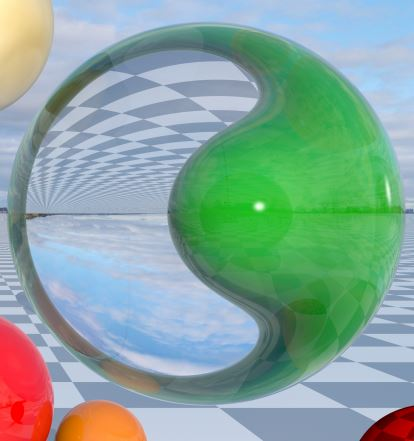
\includegraphics[scale=0.8]{img/rt/refractions.jpg}
   \end{center}
   \caption{Nous pouvons observer une boule verte à travers la boule transparente ainsi que le paysage qui est inversé à cause de la réfraction}
\end{figure}
